% definiert einen neuen Counter für die Anforderungen
\newcounter{requirementf} 
% Definiert ein neues Command für die Ausgabe der Anforderungen 
% Req Anforderungsnummer_aus_Counter: Text der Anforderung
\newcommand{\requirementf}[1]{%
\refstepcounter{requirementf}
\emph{FReq~\arabic{requirementf}:~#1}} 

% definiert einen neuen Counter für die Anforderungen
\newcounter{requirementnf} 
% Definiert ein neues Command für die Ausgabe der Anforderungen 
% Req Anforderungsnummer_aus_Counter: Text der Anforderung
\newcommand{\requirementnf}[1]{%
\refstepcounter{requirementnf}
\emph{nFReq~\arabic{requirementnf}:~#1}} 

%% setzt autoref in eine \emph Umgebung
\newcommand{\reqref}[1]{%
\emph{\autoref{#1}}} 

% Präfix Req für alle Anforderungsreferenzen
\def\requirementfautorefname{FReq}
\def\requirementnfautorefname{nFReq}

\newcommand{\requirementRegistrieren}{Der Anwender muss sich selbständig in dem System registrieren können.} 
\newcommand{\requirementUniqueLoginEmail}{Der Anwender hat nicht die Möglichkeit sich mit einem Nutzernamen oder einer E-Mail-Adresse, welche bereits im System bestehen, zu registrieren.} 
\newcommand{\requirementLogin}{Der Anwender muss sich in das System mit Nutzername und Passwort einloggen können.}
\newcommand{\requirementZugriffAufEigeneWidgets}{Dem Anwender darf nur Zugriff auf die zu seinem Account gehörigen Work"-spaces und Widgets gewährt werden.} 
\newcommand{\requirementLogout}{Der Anwender muss sich aus dem System ausloggen können.}
\newcommand{\requirementKeinZugriffNachLogout}{Nach Beendigung der Anwender-Session darf kein Zugriff mehr auf die Daten des Anwenders bestehen.}
\newcommand{\requirementWorkspaceAdd}{Der Anwender muss neue Work"-spaces in seine Lernumgebung einfügen können.}
\newcommand{\requirementWorkspaceEdit}{Der Anwender muss den Namen des Work"-spaces ändern können.}
\newcommand{\requirementWorkspaceDelete}{Der Anwender muss einen Workspace löschen können.}
\newcommand{\requirementWidgetAdd}{Der Anwender muss über ein Auswahlfeld Widgets zu Work"-spaces hinzufügen können.}
\newcommand{\requirementWidgetFilterName}{Der Anwender muss die zur Auswahl stehenden Widgets über ein Suchfeld einschränken können.}
\newcommand{\requirementWidgetFilterOnline}{Der Anwender muss die zur Auswahl stehenden Widgets so einschränken können, dass in der Liste nur offline fähige Widgets vorkommen.}
\newcommand{\requirementWidgetDelete}{Der Anwender muss ein Widget löschen können.}
\newcommand{\requirementWidgetSortDragNDrop}{Der Anwender muss in der Lage sein Widgets nach seinen Wünschen über einen Drag and Drop Mechanismus auf dem Workspace zu sortieren.}
\newcommand{\requirementWidgetInformSystem}{Die Widgets müssen dem System Informationen mitteilen können, welche Aufschluss über ihren Zustand geben.}
\newcommand{\requirementWidgetInformUser}{Die Informationen, die die Widgets dem System mitteilen, müssen dem Anwender dargestellt werden.}
\newcommand{\requirementDashboard}{Das System muss dem Anwender eine Übersichtsseite über die verwendeten Work"-spaces und Widgets und ihre wichtigsten Informationen zur Verfügung stellen.}
\newcommand{\requirementCheckOnlineStatus}{Das System muss seinen Onlinestatus kennen und bemerken, wenn sich dieser ändert.}
\newcommand{\requirementOnlineStatusInformUser}{Der Anwender muss über eine Änderung des Onlinestatus informiert werden.}
\newcommand{\requirementOfflineStart}{Das System muss für die Applikation notwendigen Ressourcen zwischenspeichern, so dass es auch offline gestartet werden kann.}
\newcommand{\requirementOfflineWork}{Das System muss den Anwender in die Lage versetzen mit den gewählten Services, zumindest rudimentär, offline zu arbeiten.}
\newcommand{\requirementOnlineSync}{Bei einer Verbindung mit dem Internet müssen die offline vorgenommenen Arbeiten mit den Services synchronisiert werden.}
\newcommand{\requirementAggregator}{Das System muss als Aggregator für unterschiedliche externe Kanäle und Services dienen und dem Anwender die Arbeit mit ihnen an zentraler Stelle ermöglichen.}
\newcommand{\requirementWidgetStandard}{Die Services müssen über einen frei verfügbaren Standard in das System eingebunden werden können.}
\newcommand{\requirementUsbStick}{Die durchgeführten Arbeiten müssen offline zwischen unterschiedlichen Rechnern transportiert werden können.}
\newcommand{\requirementUsageInBrowser}{Das System muss in aktuellen Browsern mit nativen Browsertechnologien ohne weitere Installation nutzbar sein.}
\newcommand{\requirementExtensibility}{Das System muss einfach erweitert werden können.}
\newcommand{\requirementNewWidgetsWithApi}{Es muss möglich sein über eine \ac{API} oder eine vorgegebene Implementierung neue Services und Kanäle mit offline Fähigkeiten in das System zu laden.}
\newcommand{\requirementExampleWidget}{Es muss ein offline fähiges Widget entwickelt werden, welches die offline Funktionalitäten beispielhaft umsetzt.}
\newcommand{\requirementOpenSource}{Es dürfen keine proprietären, sondern nur freie Technologien für die Umsetzung des Systems genutzt werden.}

\chapter{Anforderungsanalyse}\label{chapter:Kapitel3}  

Das Ziel der vorliegenden Arbeit ist die prototypische Implementierung einer leichtgewichtigen \ac{PLE} mit offline Fähigkeiten auf Basis aktueller Technologien. Das vorliegende Kapitel beginnt mit dem Aufbau eines möglichen Szenarios, in dem die zu entwickelnde \ac{PLE} zum Einsatz kommt. Auf Basis dieses Szenarios werden im folgenden Abschnitt Anwendungsfälle definiert. Aus den Anwendungsfälle werden die funktionalen Anforderungen an das System abgeleitet. Anschließend werden die nichtfunktionale Anforderungen definiert. Das Kapitel schließt mit einer tabellarischen Auflistung der funktionalen und nichtfunktionalen Anforderungen. 

\section{Szenario}\label{section:szenario}
Das in diesem Abschnitt vorgestellte Szenario beschreibt einen möglichen Anwendungsfall für die Arbeit mit einer \ac{PLE} und dient als Basis für die Anforderungen des in dieser Arbeit zu entwickelnden Systems. Das Szenario handelt von vier Akteuren, die sich alle von unterschiedlichen Orten aus an einem Universitätskurs beteiligen. Diese Akteure sind: ein Dozent mit Sitz in Hagen, Student 1 mit Sitz in Kamerun (Fernuni Hagen), Student 2 mit Sitz in Kamerun (Fernuni Hagen), Student 3 mit Sitz in Berlin (Fernuni Hagen) und Student 4 mit Sitz in Osnabrück (Universität Osnabrück).

Der Dozent betreut an der Fernuni Hagen unter anderem den Kurs "`E-Learning: A new approach"'. Das Ziel dieses Kurses ist die Lerntheorie des Konnektivismus (siehe \ref{section:konnektivismus}) unter Einsatz aktueller Technologien und Medien, wie beispielsweise sozialer Netze, in einem realen Umfeld zum Einsatz zu bringen. Für diesen Kurs hat der Dozent mehrere Services zur Kommunikation angelegt und den Studenten eine \ac{PLE} zur Verfügung gestellt, in der sie diese Services zusammenfassen können. Die Studenten sollen die Services wählen, die ihren Arbeitsgewohnheiten am meisten entsprechen. Am Ende des Semesters soll es eine Auswertung geben, welche Services am häufigsten genutzt und welche von den Studenten eher ignoriert wurden. Zusätzlich dazu werden die Systeme der Fernuni zur online Bearbeitung der Einsendeaufgaben genutzt. Der Dozent hat verschiedene Kommunikationskanäle angelegt. Dazu gehören: ein Twitter Kanal, ein eigener Google-Calendar, ein Chat, ein System zur Hinterlegung von Todo-Listen und ein eigener Blog, welcher einen \acsu{RSS}"=Feed (\acl{RSS}) bereitstellt. Die Studenten sind angehalten sich regelmäßig über Aktualisierungen der Services auf dem Laufenden zu halten. Für diesen Kurs haben sich die Studenten 1 und 3 eingeschrieben.

Zusätzlich haben sich Student 1, 2 und 4 zu einer virtuellen Lerngruppe zum Thema Datenbanken zusammengeschlossen. Hierfür können nicht die Systeme der Fernuni Hagen genutzt werden, da nur Student 2 momentan in dem spezifischen Kurs eingeschrieben ist. Student 1 hat sich nicht für den Kurs angemeldet und Student 4 hat überhaupt keine Möglichkeit dazu, da er nicht an der Fernuni immatrikuliert ist. Die Studenten haben sich dazu entschlossen, primär einen Chat zur Kommunikation zu benutzen.

Student 1 und Student 2 leben in Kamerun. Beide haben dort das Problem, dass der Internetzugriff aus mehreren Gründen nicht immer gegeben ist. Student 1 hat zu Hause keinen Internetzugang. Er hat nur die Möglichkeit sich mit dem Internet in der Universität oder in einem Internetcafe zu verbinden. Student 2 hat einen Internetzugang, allerdings ist dieser relativ langsam und wird nach Zeit abgerechnet, so dass es vorteilhaft für ihn ist, wenn er nur für kurze Zeit online ist. Aus diesen Gründen benötigen die beiden idealerweise ein System, welches ihnen die Möglichkeit bietet die neuesten Informationen auch offline zu lesen und zumindest rudimentär auch offline kleine Aufgaben zu erledigen. Dieses sollte sich bei Wiederverbindung mit dem Internet mit den entsprechenden Services synchronisieren. Des Weiteren sollten die Studenten in der Lage sein, die Daten auch ohne Internetverbindung zwischen verschiedenen Rechnern auszutauschen. Insbesondere Student 1 sollte die Möglichkeit haben seine Aktionen bei sich zu Hause vorzunehmen und die durchgeführten Änderungen dann an einem Rechner mit Internetanschluss zu synchronisieren. Die Anforderungen von Student 3 sind ähnlich gelagert. Er ist sehr viel unterwegs und erledigt daher viele kurze Aufgaben mit dem Smartphone. Auch hier ist eine Internetverbindung nicht immer gewährleistet oder sie wird temporär deaktiviert, um die Akkulaufzeit zu verlängern. Durch die Arbeit an unterschiedlichen Rechnern mit potentiell unterschiedlichen Betriebssystemen, ist die Installation einer komplexen Software nicht ohne Weiteres möglich. Wie durch diese kurze Beschreibung deutlich wird, haben die Teilnehmer dieses Kurses verschiedene Ausgangssituationen und damit auch spezifische Anforderungen an eine \ac{PLE}. Die \ac{PLE}, die für diese Arbeiten genutzt wird, muss also diesen Anforderungen gerecht werden und den Studenten erlauben die benötigten Services und Applikationen so zusammenzustellen wie es ihren Ansprüchen entspricht. Mögliche Arbeitsabläufe werden in Anhang \ref{AppendixD} ausführlich beschrieben. Betreuer und Studenten kommunizieren über unterschiedliche Services miteinander. Es müssen Termine geplant oder auch Notizen und Nachrichten hin und hergeschickt werden. Diese Services sollen auf einem zentralen Zugang so zusammengefasst sein, dass die Teilnehmer des Kurses alle relevanten Informationen an einer Stelle aufrufen und bearbeiten können. Dabei sind die Teilnehmer zu unterschiedlichen Zeiten online. Die Teilnehmer sollen das System offline nutzen können, um einfache Arbeiten wie das Schreiben von Twitter-Nachrichten, Notizen und Instant-Messaging Nachrichten oder eine Terminabsprache über einen Kalender erledigen zu können. Bei dem Wechsel zwischen online und offline müssen die Daten synchronisiert werden. Idealerweise haben die Nutzer alle Daten auf einem USB-Stick bei sich und können so von unterschiedlichen Rechnern, wie beispielsweise in der Universität, im Internetcafe oder zu von Hause aus, arbeiten.

\section{Funktionale Anforderungen / Anwendungsfälle}\label{section:anwendungsfaelle}
In diesem Abschnitt werden die Anwendungsfälle und die daraus resultierenden funktionalen Anforderungen beschrieben. Abbildung \ref{fig:anwendungsfaelle} zeigt Anwendungsfälle, die bei der Analyse des in Abschnitt \ref{section:szenario} vorgestellten Szenarios abgeleitet werden können. Die Anwendungsfälle werden im folgenden in textueller Form beschrieben. Aus diesen Beschreibungen werden dann direkt die funktionalen Anforderungen an das zu entwickelnde System abgeleitet. Die zu Beginn der Arbeit aufgestellten Anwendungsfälle in Form einer technischen Dokumentation (mit preconditions, postconditions etc.) sind in Anhang \ref{AppendixE} zu finden.

\begin{figure}[H]
  \centering
  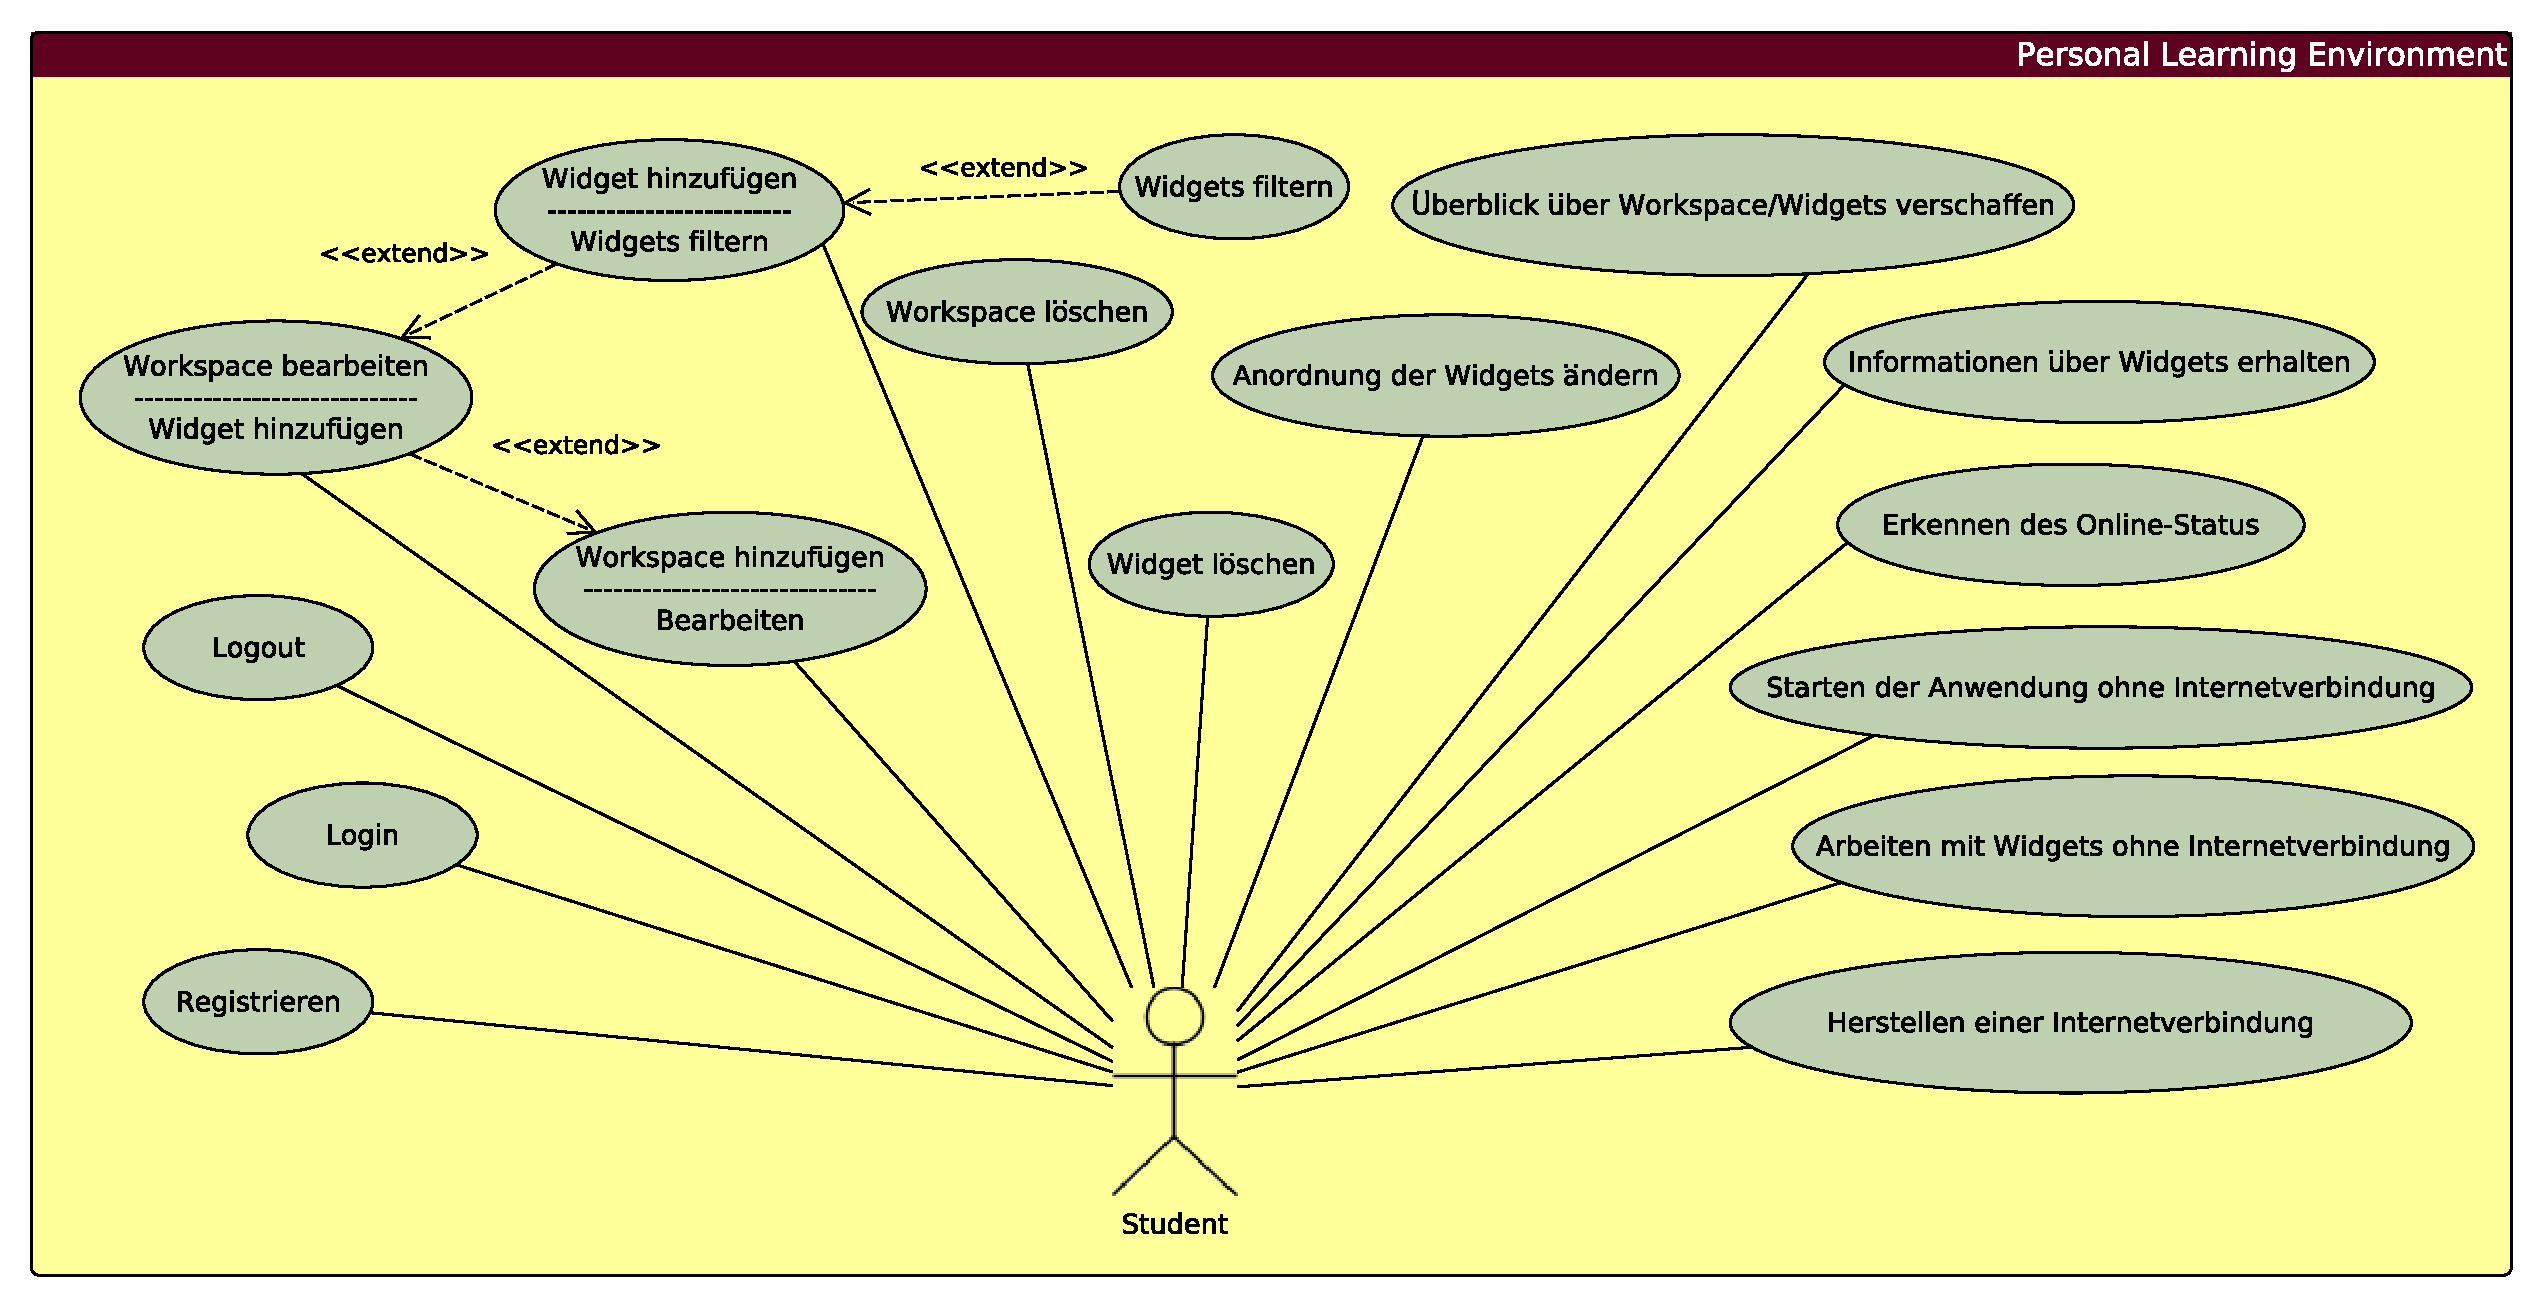
\includegraphics[width=\textwidth,height=\textheight,keepaspectratio]{./Figures/anwendungsfaelle_quer.pdf}
    \rule{35em}{0.5pt}
  \caption[Anwendungsfälle der \acs{PLE}]{Die wichtigsten Anwendungsfälle für die \acs{PLE}}
  \label{fig:anwendungsfaelle}
\end{figure}

\subsection{Anwendungsfall: Registrieren}
Der Anwender ist nicht in der \ac{PLE} registriert und erreicht erstmals die Seite des Systems. Er bekommt auf der Startseite die Möglichkeit sich für den Zugang zum System zu registrieren. Er füllt ein Formular mit seinen Daten (Vorname, Nachname, E-Mail-Adresse, Nutzername, Passwort) aus und schickt dieses Formular ab. Das System stellt bei der Anmeldung sicher, dass der Anwender sowohl Nutzername, als auch Passwort und E-Mail-Adresse eingibt und Nutzername und E-Mail-Adresse nur einmal im System vorkommen dürfen. Anschließend ist der Anwender mit seiner gewählten Nutzername-/Passwortkombination und seiner E-Mail-Adresse im System hinterlegt und kann sich somit in das System einloggen. Aus diesem Anwendungsfall folgen die funktionalen Anforderungen \reqref{requirementRegistrieren} und \reqref{requirementUniqueLoginEmail}:\\
\begin{itemize}
 \item \requirementf{\requirementRegistrieren}\label{requirementRegistrieren}
 \item \requirementf{\requirementUniqueLoginEmail}\label{requirementUniqueLoginEmail}
\end{itemize}
 
\subsection{Anwendungsfall: Login}
Ist der Anwender im System registriert, bekommt er auf der Startseite die Möglichkeit sich im System anzumelden. Er füllt ein Formular mit seiner Nutzername"=/Passwortkombination aus und schickt das Formular ab. Der Anwender ist anschließend im System eingeloggt und das System präsentiert ihm eine Übersicht über seine aktuellen Work"-spaces samt der darauf befindlichen Widgets und die wichtigsten aggregierten Informationen. Aus diesem Anwendungsfall folgen die funktionalen Anforderungen \reqref{requirementLogin} und \reqref{requirementZugriffAufEigeneWidgets}:
\begin{itemize}
 \item \requirementf{\requirementLogin}\label{requirementLogin}
 \item \requirementf{\requirementZugriffAufEigeneWidgets}\label{requirementZugriffAufEigeneWidgets}
\end{itemize}

\subsection{Anwendungsfall: Logout}
Wenn der Anwender eingeloggt ist, kann er die Aktion "`Logout"' auswählen. Anschließend wird er auf die Login-Seite weitergeleitet. Die aktuelle Session des Anwenders ist beendet und es ist ihm, ohne einen weiteren Login, nicht möglich, auf seine Daten zuzugreifen. Aus diesem Anwendungsfall folgen die funktionale Anforderung \reqref{requirementLogout} und \reqref{requirementKeinZugriffNachLogout}:
\begin{itemize}
 \item \requirementf{\requirementLogout}\label{requirementLogout}
 \item \requirementf{\requirementKeinZugriffNachLogout}\label{requirementKeinZugriffNachLogout}
\end{itemize}

\subsection{Anwendungsfall: Workspace hinzufügen}
Der Anwender wählt die Aktion "`Workspace hinzufügen"'. Hierdurch öffnet sich ein neuer Bereich, welcher einen neuen Workspace repräsentiert. Der Anwender hat nun die Möglichkeit den Workspace nach seinen Wünschen anzupassen. Nach dem Speichern wurde dem System des Anwenders ein neuer Workspace hinzugefügt. Aus diesem Anwendungsfall folgt die funktionale Anforderung \reqref{requirementWorkspaceAdd}:
\begin{itemize}
 \item \requirementf{\requirementWorkspaceAdd}\label{requirementWorkspaceAdd}
\end{itemize}
 
\subsection{Anwendungsfall: Workspace bearbeiten}
Der Anwender wählt bei einem Workspace die Aktion "`Workspace bearbeiten"'. Er hat nun die Möglichkeit den Workspace nach seinen Wünschen zu benennen und kann Widgets zu dem Workspace hinzufügen. Nach dem Speichern wurde der Workspace nach den Vorstellungen des Anwenders angepasst. Aus diesem Anwendungsfall folgt die funktionale Anforderung \reqref{requirementWorkspaceEdit}:
\begin{itemize}
 \item \requirementf{\requirementWorkspaceEdit}\label{requirementWorkspaceEdit}
\end{itemize}
 
\subsection{Anwendungsfall: Workspace löschen}
Der Anwender wählt bei einem Workspace die Aktion "`Workspace löschen"'. Es erscheint eine Rückfrage, welche eine Bestätigung des Löschvorganges (mitsamt aller Widgets) erfragt. Bei positiver Rückmeldung löscht das System den Workspace samt der zugehörigen Widgets und informiert den Anwender darüber. Aus diesem Anwendungsfall folgt die funktionale Anforderung \reqref{requirementWorkspaceDelete}:
\begin{itemize}
 \item \requirementf{\requirementWorkspaceDelete}\label{requirementWorkspaceDelete}
\end{itemize}

\subsection{Anwendungsfall: Widget hinzufügen}
Der Anwender befindet sich in einem Workspace und wählt die Aktion "`Widget hinzufügen"' Es erscheint eine Maske, in der die zur Verfügung stehenden Widgets ausgewählt werden können. Der Anwender wählt das gewünschte Widget aus und fügt es dem Workspace hinzu. Wenn gewünscht kann der Anwender die Liste der Widgets über Suchfilter einschränken. Nach dem Speichern wurde das Widget dem Workspace hinzugefügt. Aus diesem Anwendungsfall folgt die funktionale Anforderung \reqref{requirementWidgetAdd}:
\begin{itemize}
 \item \requirementf{\requirementWidgetAdd}\label{requirementWidgetAdd}
\end{itemize}

\subsection{Anwendungsfall: Widgets filtern}
Der Anwender ist dabei einem Workspace ein Widget hinzuzufügen. Er gibt in einem Textfeld eine Zeichenkette an, nach der im Namen des Widgets gesucht wird. Des Weiteren kann er in einem binären Filter wählen, ob er nur Widgets angezeigt bekommen möchte, die in der Lage sind in einem Offline-Modus zu arbeiten. Anschließend werden in der Liste der zur Auswahl stehenden Widgets nur noch diejenigen angezeigt, die der Filterung entsprechen. Aus diesem Anwendungsfall folgen die funktionalen Anforderungen \reqref{requirementWidgetFilterName} und \reqref{requirementWidgetFilterOnline}:
\begin{itemize}
 \item \requirementf{\requirementWidgetFilterName}\label{requirementWidgetFilterName}
 \item \requirementf{\requirementWidgetFilterOnline}\label{requirementWidgetFilterOnline}
\end{itemize}
 
\subsection{Anwendungsfall: Widget löschen}
Der Anwender befindet sich in einem Workspace und wählt bei einem Widget die Aktion "`Widget löschen"'. Es erscheint eine Rückfrage, welche eine Bestätigung des Löschvorganges erfragt. Bei positiver Rückmeldung löscht das System das Widget und informiert den Anwender darüber. Aus diesem Anwendungsfall folgt die funktionale Anforderung \reqref{requirementWidgetDelete}:
\begin{itemize}
 \item \requirementf{\requirementWidgetDelete}\label{requirementWidgetDelete}
\end{itemize}
 
\subsection{Anwendungsfall: Anordnung der Widgets ändern}
Der Anwender hat die Möglichkeit die einzelnen Widgets innerhalb eines Work"-spaces über einen Drag and Drop Mechanismus neu anzuordnen. Er wählt hierfür ein Widget mit der Maus aus und zieht es an die gewünschte Position. Anschließend hat sich die Anordnung der Widgets innerhalb des Work"-spaces nach dem Wunsch des Anwenders geändert. Aus diesem Anwendungsfall folgt die funktionale Anforderung \reqref{requirementWidgetSortDragNDrop}:
\begin{itemize}
 \item \requirementf{\requirementWidgetSortDragNDrop}\label{requirementWidgetSortDragNDrop}
\end{itemize}

\subsection{Anwendungsfall: Informationen über Widgets erhalten}
Der Anwender bewegt sich im System und erhält für jedes Widget direkt die wichtigsten Informationen. Hierzu gehören Informationen über die Anzahl neuer und die Anzahl der noch nicht mit dem Backend synchronisierten Einträge und über den Onlinestatus des Widgets. Aus diesem Anwendungsfall folgen die funktionalen Anforderungen \reqref{requirementWidgetInformSystem} und \reqref{requirementWidgetInformUser}:
\begin{itemize}
 \item \requirementf{\requirementWidgetInformSystem}\label{requirementWidgetInformSystem}
 \item \requirementf{\requirementWidgetInformUser}\label{requirementWidgetInformUser}
\end{itemize}

\subsection{Anwendungsfall: Überblick über Workspace/Widgets verschaffen}
Der Anwender wählt eine Aktion aus, die ihn zu einer Übersichtsseite innerhalb des Systems bringt. Das System leitet den Anwender auf eine Seite, welche ihm seine Work"-spaces und Widgets anzeigt und ihm die wichtigsten Informationen darüber vermittelt. Aus diesem Anwendungsfall folgt die funktionale Anforderung \reqref{requirementDashboard}:
\begin{itemize}
 \item \requirementf{\requirementDashboard}\label{requirementDashboard}
\end{itemize}

\subsection{Anwendungsfall: Erkennen des Onlinestatus}
Der Anwender ist eingeloggt und sieht auf den ersten Blick, dass das System online ist. Sowohl die Hauptapplikation, als auch die Widgets zeigen ihm dies an. Beendet der Anwender die Internetverbindung, aktualisieren sich diese Anzeigen und weisen damit den Anwender auf den veränderten Status hin. Aus diesem Anwendungsfall folgen die funktionalen Anforderung \reqref{requirementCheckOnlineStatus} und reqref{requirementOnlineStatusInformUser}:
\begin{itemize}
 \item \requirementf{\requirementCheckOnlineStatus}\label{requirementCheckOnlineStatus}
 \item \requirementf{\requirementOnlineStatusInformUser}\label{requirementOnlineStatusInformUser}
\end{itemize}

\subsection{Anwendungsfall: Starten der Anwendung ohne Internetverbindung}
Dem Anwender steht keine Internetverbindung zur Verfügung. Er öffnet seinen Browser und gibt die \acs{URL} (\aclu{URL}) der \ac{PLE} ein. Das System hat sich trotz fehlender Internetverbindung geöffnet und stellt dem Studenten das User-Interface dar. Aus diesem Anwendungsfall folgt die funktionale Anforderung \reqref{requirementOfflineStart}:
\begin{itemize}
 \item \requirementf{\requirementOfflineStart}\label{requirementOfflineStart}
\end{itemize}

\subsection{Anwendungsfall: Arbeiten mit Widgets ohne Internetverbindung}
Das System ist geladen, hat aber keine Internetverbindung. Der Anwender arbeitet mit den Widgets und kann neue Einträge etc. hinzufügen und bearbeiten. Alle Änderungen werden dem Anwender präsentiert, als wenn eine Internetverbindung bestehen würden. Die Änderungen werden vom System zwischengespeichert. Der Anwender erhält diesbezüglich eine Information. Aus diesem Anwendungsfall folgt die funktionale Anforderung \reqref{requirementOfflineWork}:
\begin{itemize}
 \item \requirementf{\requirementOfflineWork}\label{requirementOfflineWork}
\end{itemize}

\subsection{Anwendungsfall: Herstellen einer Internetverbindung}
Das System ist offline. Der Anwender hat in den Widgets Einträge hinzugefügt, bearbeitet oder gelöscht und stellt eine Verbindung mit dem Internet her. Die offline vorgenommenen Arbeiten werden mit dem jeweiligen Backend synchronisiert. Aus diesem Anwendungsfall folgt die funktionale Anforderung \reqref{requirementOnlineSync}:
\begin{itemize}
 \item \requirementf{\requirementOnlineSync}\label{requirementOnlineSync}
\end{itemize}

\section{Nichtunktionale Anforderungen}\label{section:nichtfunktionale_anforderunge}

\subsection{Voraussetzungen}
Wie in Abschnitt \ref{section:anwendungsfaelle} herausgestellt wird, gibt es verschiedene funktionale Anforderungen an das zu entwickelnde System. Wie in Kapitel \ref{chapter:Kapitel2} beschrieben sind \acp{PLE} Mashup-Anwendungen, welche unterschiedliche Anwendungen zu einem System zusammenfassen. Diese Anwendungen sind Services oder Kanäle, wie zum Beispiel Twitter, Facebook oder auch Applikationen für Todo-Listen oder Chats. Das System muss folglich als Aggregator fungieren, welcher diese Anwendungen in einer Anwendung bündelt, dem Nutzer diese in übersichtlicher Form präsentiert und ihm die Arbeit mit ihnen ermöglicht. Die in Abschnitt \ref{section:anwendungsfaelle} beschriebenen Widgets stellen hierbei die Umsetzung dieser Applikationen in der \ac{PLE} dar. Diese Widgets sollen in der Lage sein, wichtige Informationen an das System mitzuteilen, so dass diese für den Nutzer aufbereitet und zusammengefasst dargestellt werden können. Dem Nutzer sollen genügend Services für seine \ac{PLE} zur Verfügung stehen und die Entwicklung weiterer Widgets darf nicht von einer Person oder Firma abhängen. Aus diesem Grund muss für die Einbindung der Services ein frei verfügbarer Standard und keine proprietäre Schnittstelle verwendet werden. Die Daten sollen auch ohne Internetverbindung zwischen verschiedenen Rechnern ausgetauscht werden können, so dass gewisse Arbeiten an einem Rechner durchgeführt werden können, um sie dann an einem Rechner mit Internetanschluss zu synchronisieren. Dadurch, dass die Studenten an unterschiedlichen Rechnern mit potentiell unterschiedlichen Betriebssystemen arbeiten, welche zum Teil nicht in ihrem persönlichen Besitz sind, ist es für sie nicht oder nur sehr schwer möglich eine neue Software zu installieren. Aus diesem Grund soll das System mit nativen Browsertechnologien ohne weitere Installation nutzbar sein.

Somit ergeben sich die nichtfunktionalen Anforderungen \reqref{requirementAggregator}, \reqref{requirementWidgetStandard}, \reqref{requirementUsbStick} und \reqref{requirementUsageInBrowser}: 
\begin{itemize}
 \item \requirementnf{\requirementAggregator}\label{requirementAggregator}
 \item \requirementnf{\requirementWidgetStandard}\label{requirementWidgetStandard}
 \item \requirementnf{\requirementUsbStick}\label{requirementUsbStick}
 \item \requirementnf{\requirementUsageInBrowser}\label{requirementUsageInBrowser}
\end{itemize}

\subsection{Erweiterbarkeit}
In dieser Arbeit kann auf Grund der beschränkten Zeit nur eine prototypische Implementierung der Anforderungen erfolgen. Das System soll als Basis für weitere Entwicklungen und Forschungsarbeiten dienen und einfach erweitert und verändert werden können. Es muss zusätzlich als Aggregator für die unterschiedlichsten Services dienen. Es soll aus diesem Grund möglich sein, auf Basis einer vorgegebenen Implementierung oder \ac{API}, weitere Services oder Kanäle in das System zu laden, welche ebenfalls offline fähig sind und es so beständig in seiner Funktionalität zu erweitern. Als Grundlage für diese Erweiterung soll ein Widget auf Basis der \ac{API} umgesetzt werden. Dieses soll die beschriebenen offline Funktionalitäten nutzen. Schließlich wird die Software in unterschiedlichen Bereichen, insbesondere in einem universitären Umfeld eingesetzt. Dies verlangt eine Nutzbarkeit ohne Lizenzgebühren für die verwendeten Technologien, so dass für die Umsetzung keine proprietären, sondern nur freie Technologien verwendet werden dürfen. Aus diesen Punkten folgen die weiteren nichtfunktionalen Anforderungen \reqref{requirementNewWidgetsWithApi}, \reqref{requirementExampleWidget}, \reqref{requirementExtensibility}, und \reqref{requirementOpenSource}:
\begin{itemize}
 \item \requirementnf{\requirementNewWidgetsWithApi}\label{requirementNewWidgetsWithApi}
 \item \requirementnf{\requirementExampleWidget}\label{requirementExampleWidget}
 \item \requirementnf{\requirementExtensibility}\label{requirementExtensibility}
 \item \requirementnf{\requirementOpenSource}\label{requirementOpenSource}
\end{itemize}

\section{Überblick über die Anforderungen}
In den vorherigen Abschnitten wurden nichtfunktionale und funktionale Anforderungen an das zu entwickelnde System aufgestellt und beschrieben. In den folgenden zwei Tabellen sind diese Anforderungen noch einmal zusammengefasst.

\renewcommand{\arraystretch}{1.4} % Tabellenabstände vergrößern
\begin{table}[ht]
\caption{Funktionale Anforderungen}
\begin{tabularx}{\textwidth}{ l | X }
\reqref{requirementRegistrieren} & \emph{\requirementRegistrieren} \\ \hline 
\reqref{requirementUniqueLoginEmail} & \emph{\requirementUniqueLoginEmail} \\ \hline 
\reqref{requirementLogin} & \emph{\requirementLogin} \\ \hline 
\reqref{requirementZugriffAufEigeneWidgets} & \emph{\requirementZugriffAufEigeneWidgets} \\ \hline 
\reqref{requirementLogout} & \emph{\requirementLogout} \\ \hline 
\reqref{requirementKeinZugriffNachLogout} & \emph{\requirementKeinZugriffNachLogout} \\ \hline 
\reqref{requirementWorkspaceAdd} & \emph{\requirementWorkspaceAdd} \\ \hline 
\reqref{requirementWorkspaceEdit} & \emph{\requirementWorkspaceEdit} \\ \hline 
\reqref{requirementWorkspaceDelete} & \emph{\requirementWorkspaceDelete} \\ \hline 
\reqref{requirementWidgetAdd} & \emph{\requirementWidgetAdd} \\ \hline 
\reqref{requirementWidgetFilterName} & \emph{\requirementWidgetFilterName} \\ \hline 
\reqref{requirementWidgetFilterOnline} & \emph{\requirementWidgetFilterOnline} \\ \hline 
\reqref{requirementWidgetDelete} & \emph{\requirementWidgetDelete} \\ \hline 
\reqref{requirementWidgetSortDragNDrop} & \emph{\requirementWidgetSortDragNDrop} \\ \hline 
\reqref{requirementWidgetInformSystem} & \emph{\requirementWidgetInformSystem} \\ \hline 
\reqref{requirementWidgetInformUser} & \emph{\requirementWidgetInformUser} \\ \hline 
\reqref{requirementDashboard} & \emph{\requirementDashboard} \\ \hline 
\reqref{requirementCheckOnlineStatus} & \emph{\requirementCheckOnlineStatus} \\ \hline 
\reqref{requirementOnlineStatusInformUser} & \emph{\requirementOnlineStatusInformUser} \\ \hline 
\reqref{requirementOfflineStart} & \emph{\requirementOfflineStart} \\ \hline 
\reqref{requirementOfflineWork} & \emph{\requirementOfflineWork} \\ \hline 
\reqref{requirementOnlineSync} & \emph{\requirementOnlineSync} \\ \hline 
\end{tabularx}
\label{table:funktionale_anforderungen}
\end{table}

\clearpage % damit die Tabelle oben erscheint
\begin{table}[ht!]
\caption{Nichtfunktionale Anforderungen}
\begin{tabularx}{\textwidth}{ l | X }
\reqref{requirementAggregator} & \emph{\requirementAggregator} \\ \hline 
\reqref{requirementWidgetStandard} & \emph{\requirementWidgetStandard} \\ \hline 
\reqref{requirementUsbStick} & \emph{\requirementUsbStick} \\ \hline 
\reqref{requirementUsageInBrowser} & \emph{\requirementUsageInBrowser} \\ \hline 
\reqref{requirementNewWidgetsWithApi} & \emph{\requirementNewWidgetsWithApi} \\ \hline 
\reqref{requirementExampleWidget} & \emph{\requirementExampleWidget} \\ \hline
\reqref{requirementExtensibility} & \emph{\requirementExtensibility} \\ \hline 
\reqref{requirementOpenSource} & \emph{\requirementOpenSource} \\ \hline 
\end{tabularx}
\label{table:nichtfunktionale_anforderungen}
\end{table}

